\PassOptionsToPackage{ukrainian,english}{babel}
\documentclass[twocolumn]{el-author}

%\usepackage[...]{...}      This has been commented out as we are not using any additional packages here.  On the whole, they should be unnecessary.
\usepackage{mathtext}
\usepackage[T1,T2A]{fontenc}
\usepackage[english,ukrainian]{babel}
\usepackage{hyperref}
\usepackage{graphicx} %package to manage images
\usepackage[a4paper, total={7in, 9.5in}]{geometry}
\usepackage{makecell}
\graphicspath{ {images/} }
\newcommand{\hH}{\hat{H}}
\newcommand{\D}{^\dagger}
\newcommand{\ua}{\uparrow}
\newcommand{\nc}{\newcommand}
\renewcommand\theadfont{\normalsize\scshape}
\nc{\da}{\downarrow} \nc{\hc}{\hat{c}} \nc{\hS}{\hat{S}}
\nc{\bra}{\langle} \nc{\ket}{\rangle} \nc{\eq}{equation (\ref}
\nc{\h}{\hat} \nc{\hT}{\h{T}}\nc{\be}{\begin{eqnarray}}
\nc{\ee}{\end{eqnarray}}\nc{\rd}{\textrm{d}}\nc{\e}{eqnarray}\nc{\hR}{\hat{R}}\nc{\Tr}{\mathrm{Tr}}
\nc{\tS}{\tilde{S}}\nc{\tr}{\mathrm{tr}}\nc{\8}{\infty}\nc{\lgs}{\bra\ua,\phi|}\nc{\rgs}{|\ua,\phi\ket}
\nc{\hU}{\hat{U}}\nc{\lfs}{\bra\phi|}\nc{\rfs}{|\phi\ket}\nc{\hZ}{\hat{Z}}\nc{\hd}{\hat{d}}\nc{\mD}{\mathcal{D}}
\nc{\bd}{\bar{d}}\nc{\bc}{\bar{c}}\nc{\mc}{\mathcal}\nc{\ea}{eqnarray}\nc{\mG}{\mathcal{G}}\nc{\bce}{\begin{center}}
\nc{\ece}{\end{center}}
\date{20 Грудня 2018}

\begin{document}

\title{Вивчення будови та принципу дії газових квантових генераторів}

\author{Сергій Поліщук}

\maketitle

\section{Мета роботи}

Вивчення будови та принципу дії газових квантових генераторів

\section{Прилади і матеріали}

оптична лава, гелій-неоновий лазер, дифракційна
гратка, міліметровий папір, рулетка, поляроїд, екран з
короткофокусною лінзою, скляна плоскопаралельна
пластинка.

\section{Завдання}

\begin{enumerate}
	\item при домашній підготовці:
	\begin{itemize}
		\item  ознайомитись з фізичними основами будови та принципу дії
оптичних квантових генераторів;
		\item  згідно з рекомендаціями до роботи виготовити
комп'ютерним способом на прозорій плівці декілька
дифракційних решіток з різним періодом;
	\end{itemize}
	\item при виконанні роботи:
	\begin{itemize}
		\item  дослідити лазерне випромінювання на поляризованість;
		\item  визначити сталу досліджуваної решітки;
		\item  визначити час когерентності лазерного випромінювання;
		\item  визначити плоский кут розходження лазерного
випромінювання.
	\end{itemize}
	
\end{enumerate}

\section{Правила техніки безпеки}

\begin{itemize}
	\item  не вмикати і не вимикати лазер самостійно -- висока
напруга;
	\item  ні в якому разу не дивіться назустріч лазерному променю --
можете пошкодити очі.
\end{itemize}

\section{Теоретичні відомості та опис установки}

Оптичний квантовий генератор (лазер) - прилад, у якому здійснюється
генерація монохроматичних електромагнітних хвиль оптичного діапазону в
результаті індукованого випромінювання. Слово «лазер» складено із
початкових літер англійських слів Light Amplification by Stimulated Emission of Radiation.

Оптичні квантові генератори -- це унікальні, штучно створені,
принципово нові джерела світла, які володіють високою когерентністю і
монохроматичністю. Крім того, випромінювання лазера поляризоване. Ще
однією важливою характеристикою цих приладів є вузька спрямованість їх
випромінювання. Із-за дифракції кут розходження променів не може бути
меншим $\frac{\lambda}{d}$, де $d$ - ширина пучка. 
У лазерах ця гранична межа майже досягнута.

Перші квантові генератори були створені М.~Г.~Басовим і О.~М.~Прохоровим 
та незалежно від них Ч.~Таунсом у 1955~році (Нобелівська
премія 1964~р.). Фізичні принципи їх роботи основані на квантових
закономірностях. Із них слідує, що кожному стану системи відповідає певна
енергія. Якщо квантова система не піддається зовнішньому впливу, то вона
інаходиться у стаціонарному стані з найменшою енергією $E_{1}$. За рахунок
пенних зовнішніх чинників систему можна перевести у збуджений стан з
енергією $E_{2}$. Такий стан є нестійким, його тривалість не перевищує $10^{-9}$с, 
без будь-якого зовнішнього впливу система здійснить перехід у стан з меншою
енергією $E_{1}$, випромінюючи при цьому фотон з частотою $v$: $hv = E_{2} - E_{1}$.

Такий самодовільний (спонтанний) перехід, а, отже, і випромінювання,
має випадковий, ймовірносний характер, передбачити, коли він відбудеться,
принципово неможливо. Це означає, що атоми випромінюють незалежно і
неодночасно, фази випромінюваних ними електромагнітних хвиль не
утгоджені між собою. Випадковими є не лише моменти випромінювання
фотонів, а й напрямки їх поширення і поляризації. Так випромінюють
звичайні джерела світла, таке випромінювання неполяризоване, некогерентнє
і меспрямоване.

У 1916~році А.~Ейнштейн теоретично показав, що за пєвних умов
процесом переходу атома з рівня $E_{2}$, на рівень $E_{1}$, все ж таки можна керувати.
Такий керований (індукований) перехід можна здійснити за допомогою
електромагнітної хвилі, частота якої рівна, або достатньо близька до частоти
$v = \frac{(E_{2} - E_{1})}{h}$.
У цьому випадку зовнішній фотон, який стимулює збуджену
систему до випромінювання, і фотони, що цією системою випромінюються,
будуть абсолютно тотожні -- вони матимуть однакову частоту і фазу
коливань, той же напрям поширення і ту ж поляризацію.

Для реалізації такого механізму підсилення світла необхідно, щоб
число індукованих переходів з випромінюванням фотонів було більшим
числа переходів з поглинанням фотонів тієї ж частоти , а для цього потрібно,
щоб число атомів у збудженому стані, у стані з більшою енергією було б
більшим числа атомів з меншою енергією. Таке положення систєми не є
природним, воно одержало назву інверсного (лат. inversio - перестановка),
термодинамічно такий стан нестабільний (стан з від'ємною температурою).
Проте за певних умов система у такому стані може перебувати достатньо
лдонго, значно довше, ніж $10^{-8}$с. Середовище з інверсним заселенням
енергетичних рівнів називають активним. Одержати активне середовище
можна кількома способами: у твердотільних лазерах - це оптичне
підкачування, у газових - електричний розряд, у напівпровідникових -
інжекція носіїв тощо.

\begin{figure}[h]
\centering{\includegraphics[width=80mm]{img_1}}
\caption{\source{}}
\label{img:1}
\end{figure}

Активною квантова система буде лише тоді, коли вона матиме
нетастабільний рівень -- рівень, на якому електрони можуть перебувати
значний час. Цей час у $10^{5}$ разів більший, ніж час перебування електронів на
інших рівнях збудженого атома. Утворюється метастабільний рівень за
рихунок введення в основну робочу речовину спеціально підібраних
домішок. У рубіновому лазері -- це атоми хрому, у гелій-неоновому -- атоми
гелію, Важливою умовою добору пари основа-домішка є розміщення
нетастабільного рівня дещо нижче енергетичних рівнів збуджених атомів
основи. У результаті такого розташування утворюється система, спрощений
вигляд якої зображений на рис.\ref{img:1}. У цій схемі метастабільним є рівень 2. За рахунок підкачування частину електронів переводять з нижнього
енергетичного рівня 1 на рівень 3. При цьому, поряд з оберненим переходом
$3 \to 1$, без випромінювання відбувається перехід $3 \to 2$. Оскільки час життя
електронів на рівні 2 значний (до $10^{-3}$с), то підкачуванням можна домогтися
такого стану, коли заселення енергетичного рівня 2 перевищуватиме
заселення енергетичного рівня 1 - станеться інверсія заселеності рівня 2 по
відношенню до рівня 1. Незначна зовнішня дія (фотон з частотою
$v = \frac{(E_{2} - E_{1})}{h}$ 
спричинить значну кількість вимушених (з випромінюванням)
переходів $2 \to 1$ - відбудеться підсилення світла.

\begin{figure}[h]
\centering{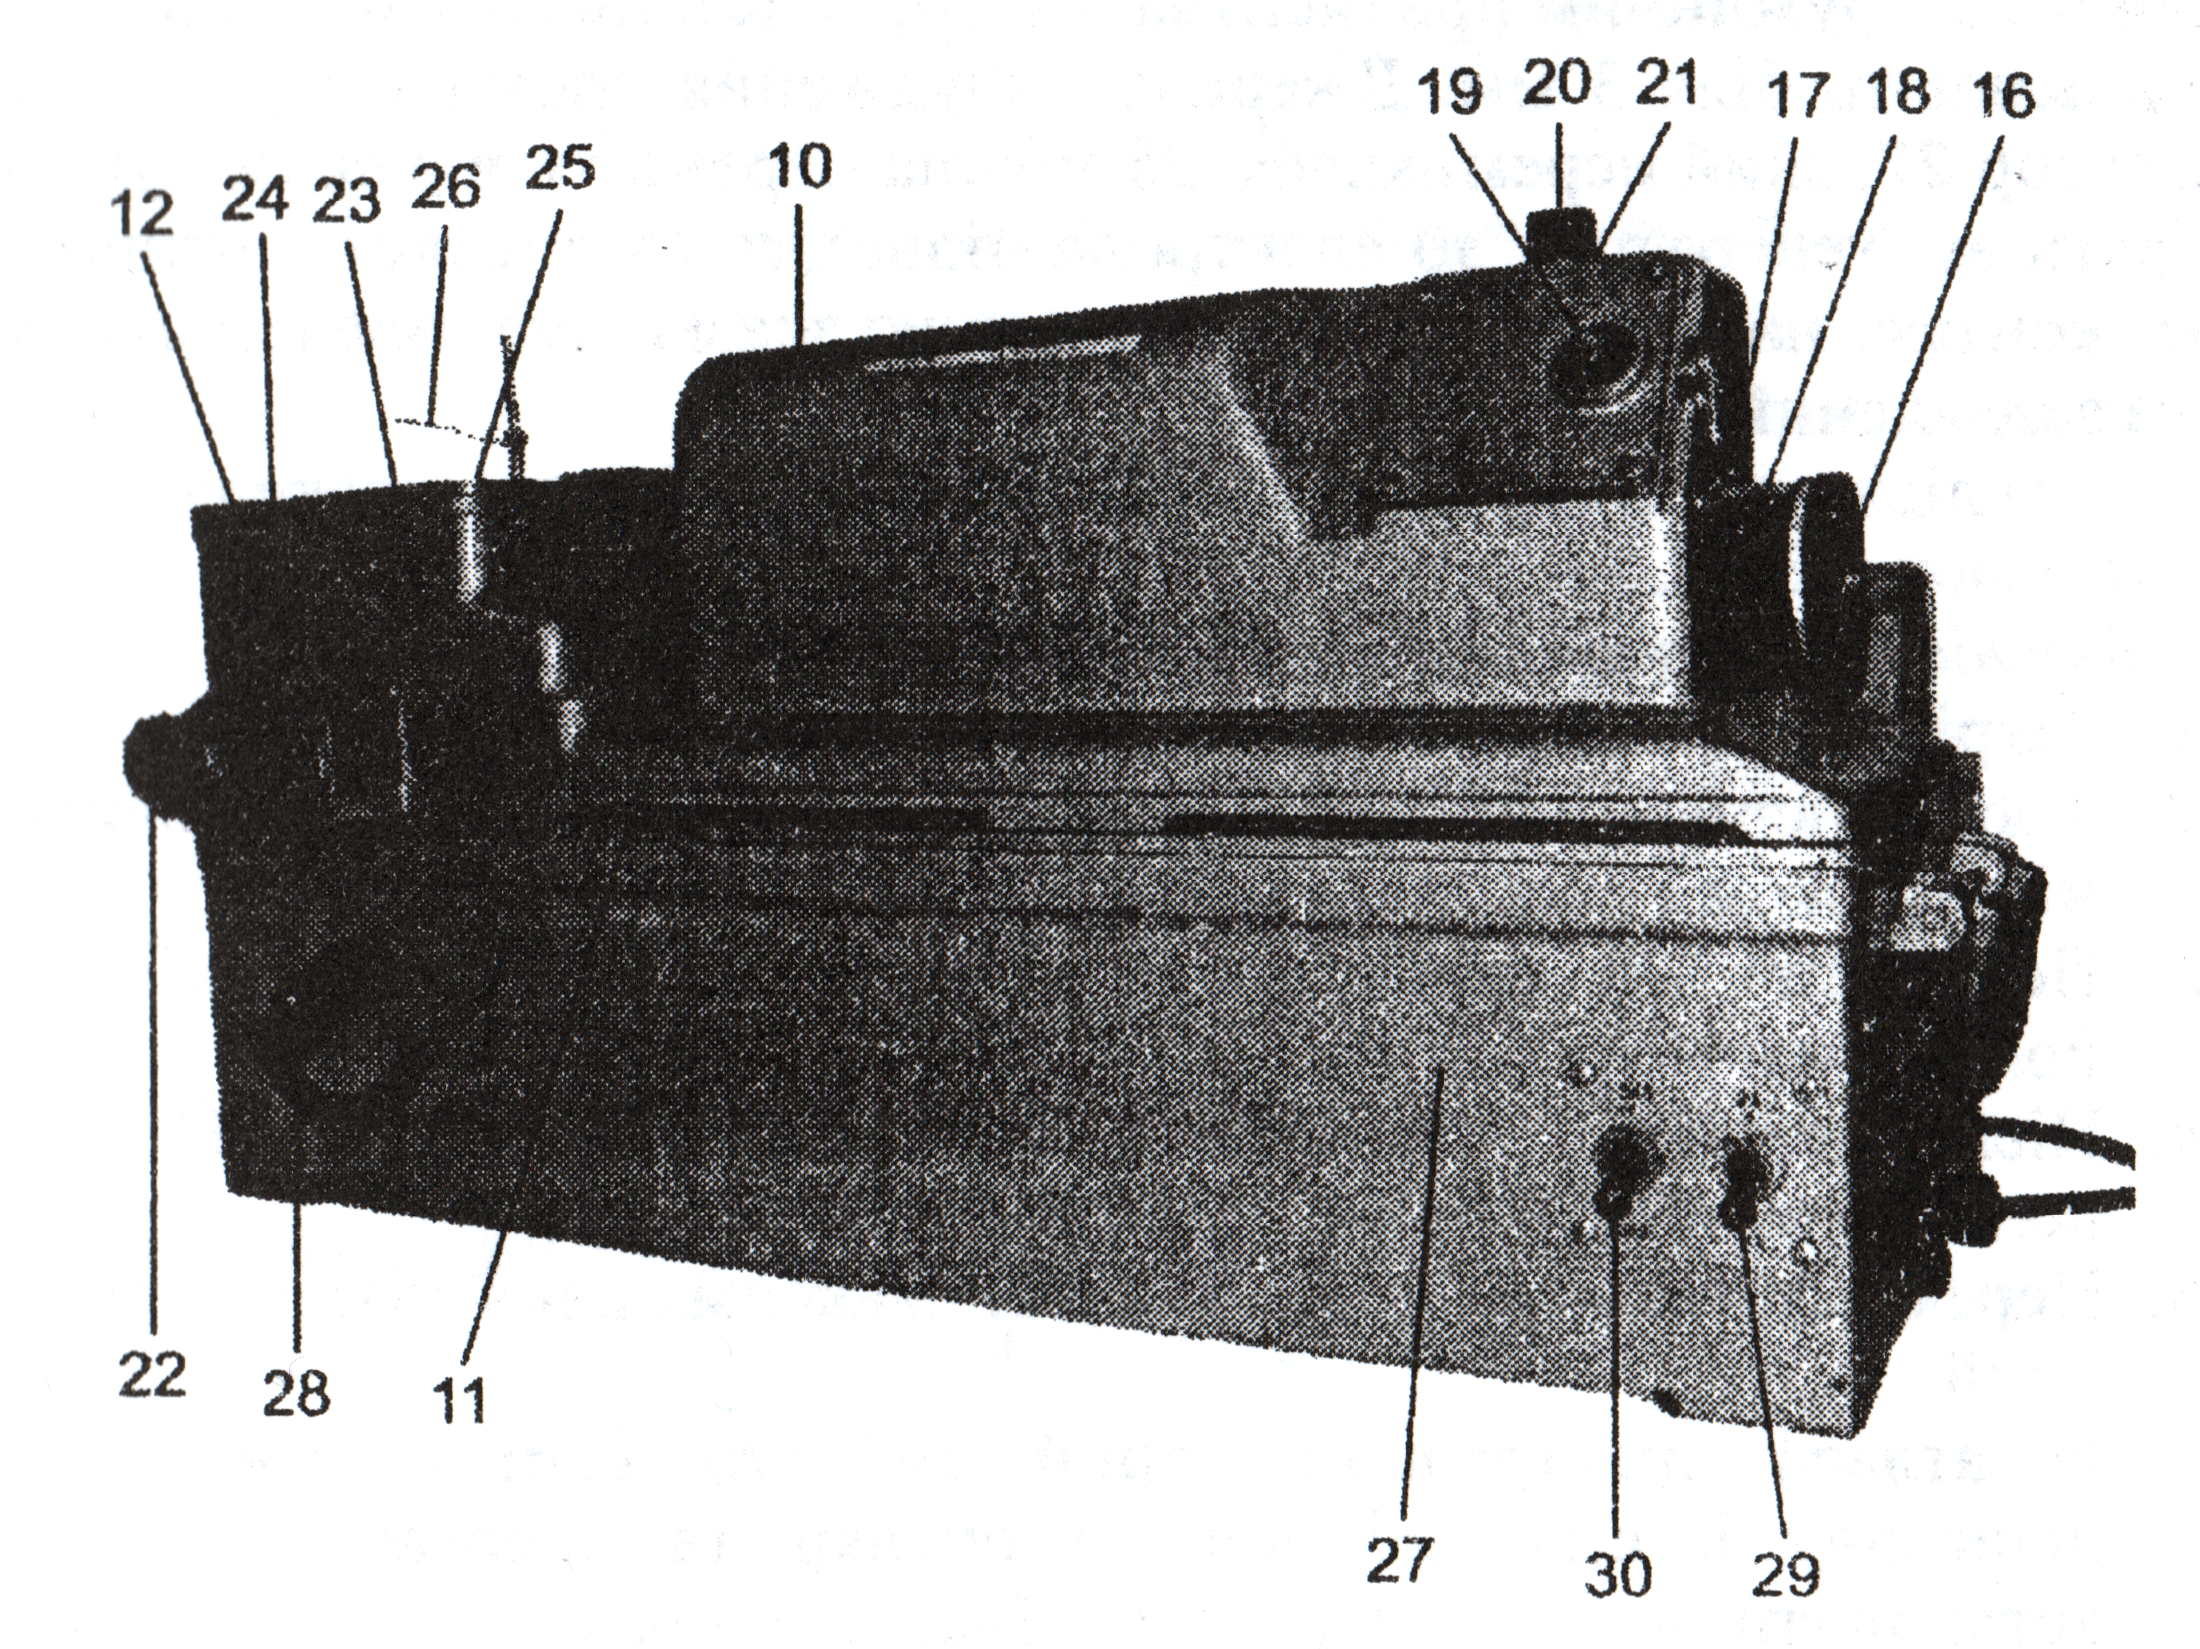
\includegraphics[width=80mm]{img_2}}
\caption{\source{}}
\label{img:2}
\end{figure}

У реальних оптичних генераторах кількість рівнів, зазвичай, більша, ніж три,
проте суть процесів, що мають при цьому місце, однакова - метод трьох
рівнів універсальний. Розглянемо, наприклад, принцип дії гелій-неонового
лазера. Схема енергетичних рівнів для нього зображена на рис.\ref{img:2}. 
Гелій має
два метастабільні рівні $E_{2}^{1}$ і $E_{3}^{1}$, 
на яких електрони перебувають значний час --
$10^{-3}$с, тому концентрація збуджених атомів гелію у електричному розряді
дуже велика. Принциповою особливістю енергетичних рівнів атомів гелію і
неону є дуже близьке розташування метастабільних рівнів $E_{2}^{1}$ і $E_{3}^{1}$; гелію та
відповідно рівні $E_{2}$ і $E_{3}$, атомів неону. Тому при зіткненні таких атомів
відбувається резонансна передача енергії від гелію до неону. У результаті
число атомів неону на рівнях $E_{2}$ і $E_{3}$, різко збільшується, що призводить до
інверсної заселеності рівнів $E_{2}$ і $E_{3}$, по відношенню до рівнів $E_{4}$ і $E_{5}$.
Індуковані переходи $E_{3} \to E_{4}$, $E_{3} \to E_{5}$ і $E_{2} \to E_{5}$ дають випромінювання з 
довжиною хвилі відповідно 3391~нм, 632,8~нм та 1152~нм. Підбираючи склад
нанесеного на дзеркала  відбиваючого шару, одержують лазерне
випромінювання однієї з перелічених довжин хвиль, зазвичай, це 632,8~нм.
Дліеркала виготовляють з багатошаровим діелектричним покриттям, що має
коефіцієнт відбивання 99%.

Значення дзеркал не обмежується виділенням однієї з трьох довжин
хпиль. Вони виконують ще одну важливу функцію -- слугують оптичним
резонатором, який забезпечує позитивний обернений зв'язок. Завдання
резонатора -- спрямувати частину одержаного випромінювання знову у
систему, щоб воно викликало появу нових фотонів, тобто привело до
додаткового збільшення інтенсивності світла. З цією метою газорозрядну
трубку з сумішшю гелію і неону розміщують між дзеркалами (рис.\ref{img:3}). Одне
лаеркало виготовляють сферичним, друге - плоским. Прозорість одного
близько 296, іншого менше 196. За допомогою спеціальних пристроїв
леркала встановлюють так, щоб оптична вісь сферичного дзеркала була
строго перпендикулярна плоскому дзеркалу.

\begin{figure}[h]
\centering{\includegraphics[width=80mm]{img_3}}
\caption{\source{}}
\label{img:3}
\end{figure}

Окрім забезпечення оберненого зв'язку, дзеркала ще роблять
випромінювання направленим, оскільки фотони, які не рухаються вздовж вісі
дзеркала, виходять з активного середовища через бокову поверхню,
практично без підсилення.

Торці газорозрядної трубки скошені під кутом Брюстера і закриті
окляними чи кварцовими вікнами, що забезпечує поляризацію лазерного
випромінювання.

У кварцовій газорозрядні трубці 1 знаходиться суміш газів: гелій під
тиском 1мм~рт.ст. та неон, який створює тиск 0,1~мм~рт.ст. Трубка має
підігрівний катод 2 та анод 3, між якими прикладається напруга 1-2,5 кВ.
Потужність гелій-неонових лазерів не перевищує десятків мВт. Розходження
пучка біля 20".

Перший лазер безперервної дії на суміші газів гелію і неону був
розроблений у 1961~році. У цьому лазері неон є робочою речовиною, а гелій
слугує резервуаром збуджень, які резонансно передаються атомам неону.

%\begin{table}[ht]
%\processtable{Спектральні характеристики деяких скляних світлофільтрів}
%{\begin{tabular}{|l|l|l|l|l|}\hline
%\thead{№} & 
%\thead{{\scriptsize Марка} \\ {\scriptsize світлофільтра}} & 
%\thead{{\scriptsize Товщина} \\ {\scriptsize скла, мм}} & 
%\thead{{\scriptsize Довжина хвилі} \\ {\scriptsize максимального} \\ {\scriptsize пропускання, м}} & 
%\thead{{\scriptsize Частота хвилі} \\ {\scriptsize максимального} \\ {\scriptsize пропускання, Гц}}\\\hline
%1 & КС-13 & 2,78 & $700*10^{-9}$ & $4.3*10^{14}$ \\\hline
%2 & OC-13 & 3,02 & $650*10^{-9}$ & $4.6*10^{14}$ \\\hline
%3 & ЖС-18 & 3,07 & $600*10^{-9}$ & $5.0*10^{14}$ \\\hline
%4 & 3C-1 & 1,00 & $540*10^{-9}$ & $506*10^{14}$ \\\hline
%5 & CC-2 & 1,00 & $390*10^{-9}$ & $7.7*10^{14}$ \\\hline
%6 & ФС-6 & 1,00 & $360*10^{-9}$ & $8.3*10^{14}$ \\\hline
%\end{tabular}}{}
%\end{table}

\newpage

\section{Послідовність виконання роботи}

\begin{enumerate}
	\item На оптичній лаві послідовно розташувати лазер, поляроїд і екран.
Обертаючи поляроїд, переконатись у зміні освітленості на екрані.
Це свідчить про лінійну поляризацію випромінюваного лазером
світла.
	\item На оптичній лаві замість поляроїда встановити саморобну
дифракційну решітку. Екран із закріпленим на ньому
міліметровим папером розмістити якомога далі від решітки.
Користуючись формулою $d~sin~ \phi = m \lambda$ та маючи на увазі, що при
малих $\phi$ $sin~ \phi \approx tg~ \phi = \frac{a}{l}$, визначити сталу решітки

\begin{equation} \label{eq:1}
d = m \cdot \frac{l}{a} \cdot \lambda
\end{equation}
де $l$ -- відстань від решітки до екрату, $a$ -- відстань між центральним і $m$-ним максимумами.

Вимірювання виконати декілька разів для різних $m$,
виконати обробку та аналіз результатів.
	\item Встановити на оптичній лаві екран, у центрі якого закріпити
короткофокусну лінзу від об'єктива мікроскопа. Одержаний
розбіжний пучок спрямувати на розміщену по інший бік екрану,
паралельно до нього, товсту (близько 10~мм) скляну
плоскопаралельну пластинку. На екрані, у відбитому від
пластинки світлі, будуть спостерігатися інтерференційні кільця,
що свідчить про можливість спостереження інтерференції не
лише від тонких плівок. Наявність інтерференційної картини у
товстому склі вказує на значний час когерентності лазерного
випромінювання. У даному випадку його слід оцінити за
різницею ходу променів, що інтерферують. Це промені, які
відбиваються від задньої і передньої поверхні скла. Їх різниця
ходу $\Delta \approx 2dn$, де $d$ і $n$ - відповідно товщина і показник заломлення
скла. Тоді час когерентності $r \geq \frac{\Delta}{c} = \frac{2dn}{c}$
($c$ -- швидкість світла)
	\item Спрямувати лазерний промінь спочатку на розташований на
оптичній лаві екран, а потім на віддалену стіну. За допомогою
міліметрового паперу визначити діаметри плям та виміряти
рулеткою відстані від них до лазера. Виходячи з рис.\ref{img:4}, за
формулою $\phi = \frac{(D-d)}{(L-l)}$ визначити кут розходження пучка.

\begin{figure}[h]
\centering{\includegraphics[width=80mm]{img_4}}
\caption{\source{}}
\label{img:4}
\end{figure}

	\item Експерименти повторити при різних $L$, і $l$. Визначити середнє
значення кута $\phi$.
\end{enumerate}

\newpage
\begin{thebibliography}{}

\bibitem{1}
Кучерук І.М., Горбачук І.Т. Загальний курс фізики: Т.3.: Оптика.
Квантова фізика. -К.: Техніка, 2006. - 518с., ст. 330 - 337.

\bibitem{2}
Кучерук І.М, Дущенко В.П. Загальна фізика. Оптика. Квантова
фізика. - К.: Вища школа, 1991. -- 463с., ст. 342 - 347.

\bibitem{3}
Горбачук І.Т. Загальна фізика. Лабораторний практикум. - К.:
Вища школа, 1992.- 512 с., ст. 442 - 447.

\bibitem{4}
Дущенко В.П. Фізичний практикум. - К.: Вища школа, 1984. --
256с., ст. 145 - 146.

\bibitem{5}
Методична розробка до роботи.

\end{thebibliography}

\section{Завдання для самоконтролю}

\begin{enumerate}
	\item У чому суть спонтанного та індуктивного випромінювання?
	\item Яка будова та принцип дії газового лазера?
	\item Яка будова оптичного резонатора?
	\item Яку роль відіграють домішки гелію?
	\item Яка роль атомів неону?
	\item При яких умовах відбувається генерація світла в активному
середовищі?
	\item Зарахунок чого лазерне випромінювання поляризоване?
	\item Який механізм дії трирівневої системи?
	\item Які типи оптичних квантових генераторів Вам відомі?
	\item Що таке довжина та час когерентності?
\end{enumerate}

\clearpage
\section{Тестові завдання для вхідного контролю}

\begin{enumerate}
	\item Які з нижче перелічених властивостей випромінювання притаманні лазеру:
1) монохроматичність, 2) когерентність, 3) поляризованість, 4) вузька
спрямованість, 5) висока проникна здатність, 6) дуже добре поглинання
речовинами?
	\begin{enumerate}
		\item перша, четверта і п'ята;
		\item друга, третя і шоста;
		\item всі шість;
		\item перші чотири.
	\end{enumerate}
	\item Час перебування атома у збудженому стані має порядок:
	\begin{enumerate}
		\item $10^{-3}c$;
		\item $10^{-4}c$;
		\item $10^{-6}c$;
		\item $10^{-8}c$.
	\end{enumerate}
	\item Метастабільні рівні:
	\begin{enumerate}
		\item існують у будь-якій речовині;
		\item утворюються лише в очищених речовинах;
		\item з'являються за рахунок введення в речовину певних домішок;
		\item утворюються при наявності власних дефектів у речовині.
	\end{enumerate}
	\item У гелій-неоновому лазері концентрації гелію і неону:
	\begin{enumerate}
		\item приблизно однакові;
		\item гелію значно більше;
		\item неону на порядок більше;
		\item співвідношення концентрацій може бути будь-яким.
	\end{enumerate}
	\item Активним називають середовище:
	\begin{enumerate}
		\item атоми якого знаходяться у збудженому стані;
		\item яке випромінює світло;
		\item у якому існують енергетичні рівні з інверсним заселенням;
		\item яке здатне збудити інше середовище.
	\end{enumerate}
	\item Лазери бувають: 1) твердотільні, 2) рідинні, 3) напівпровідникові, 4) газові.
Чи всі ці твердження вірні?
	\begin{enumerate}
		\item вірні 1 і 4 твердження;
		\item рідинні лазери не існують;
		\item вірні І, 2 і 4 твердження;
		\item існують всі перелічені типи лазерів.
	\end{enumerate}
	\item Гелій-неоновий лазер випромінює світло з довжиною хвилі:
	\begin{enumerate}
		\item 589нм;
		\item 623,2нм;
		\item 632,8нм;
		\item 6563нм.
	\end{enumerate}
	\item Потужність випромінювання гелій-неонових лазерів складає порядок:
	\begin{enumerate}
		\item $10^{3}Вт$;
		\item $10Вт$;
		\item $10^{-2}Вт$;
		\item $10^{-5}Вт$.
	\end{enumerate}
	\item Лазерне випромінювання: 1) когерентне, 2) синфазне, 3) монохроматичне,
4) лінійно поляризоване, 5) вузько спрямоване. Для одержання якої (яких)
з цих ознак лазерний генератор повинен мати, крім основних, ще додаткові
конструкти елементи?
	\begin{enumerate}
		\item другої та п'ятої;
		\item лише четвертої;
		\item лише третьої;
		\item першої та третьої.
	\end{enumerate}
	\item У сучасних газових лазерах час когерентності може досягати:
	\begin{enumerate}
		\item $10^{-8}c$;
		\item $10^{-6}c$;
		\item $10^{-4}c$;
		\item $10^{-2}c$.
	\end{enumerate}
\end{enumerate}

\section{Тестові завдання для підсумкового контролю}

\begin{enumerate}
	\item Лазерне випромінювання: спонтанне, індуковане, вимушене, наведене. Яке
(-і) з цих тверджень хибне (-і)?
	\begin{enumerate}
		\item перше;
		\item четверте;
		\item перше і четверте;
		\item всі твердження вірні.
	\end{enumerate}
	\item Час життя електрона на метастабільному рівні складає близько:
	\begin{enumerate}
		\item $10^{-3}c$;
		\item $10^{-1}c$;
		\item $10^{2}c$;
		\item $10^{3}c$.
	\end{enumerate}
	\item  У гелій-неоновому лазері метастабільні рівні утворюються за рахунок:
	\begin{enumerate}
		\item атомів гелію;
		\item атомів неону;
		\item атомів хрому;
		\item незначної кількості атомів повітря.
	\end{enumerate}
	\item Для утворення інверсної заселеності енергетичних рівнів необхідно, щоб:
	\begin{enumerate}
		\item метастабільні рівні розташовувалися дещо вище рівнів робочої
речовини;
		\item метастабільні рівні знаходилися значно вище рівнів робочої речовини;
		\item ті рівні, переходи з яких відбуваються з нив вчена знаходилися
вище метастабільних рівнів;
		\item кількість рівнів, переходи з яких дають внпродуитнюними перевищувала
кількість метастабільних рівнів.
	\end{enumerate}
	\item Для здійснення індукованого випромінювання необхідно задіяти наступну
кількість енергетичних рівнів:
	\begin{enumerate}
		\item достатньо двох;
		\item не менше трьох;
		\item як мінімум чотири;
		\item будь-яку.
	\end{enumerate}
	\item Збудження активного середовища можна здійснити за рахунок:
	\begin{enumerate}
		\item оптичного підкачування;
		\item електричного розряду;
		\item інжекції носіїв заряду;
		\item нагрівання.
	\end{enumerate}
	\item Яке з цих тверджень хибне?
	Найхарактернішою відмінністю лазерного випромінювання від
випромінювань інших джерел є його:
	\begin{enumerate}
		\item монохроматичність;
		\item поляризованість;
		\item когерентність;
		\item синфазність.
	\end{enumerate}
%	\item Яку(-і) з перелічених нижче функцій оптичний резонатор не здійснює:
%	1) позитивний обернений зв'язок, 2) направленість випромінювання,
%3) підсилення світлового потоку в активному середовищі, 4) поляризацію
%світла, 5) монохроматизацію світла?
%	\begin{enumerate}
%		\item другу і п'яту;
%		\item першу і третю;
%		\item четверту;
%		\item п'яту.
%	\end{enumerate}
	\item Під часом когерентності розуміють:
	\begin{enumerate}
		\item час випромінювання атомом цугу хвиль;
		\item час перебування атома у збудженому стані;
		\item час переходу атома із збудженого стану в стаціонарний;
		\item час, необхідний для інтерференції світлових хвиль.
	\end{enumerate}
\end{enumerate}
\newpage
~
\end{document}

%\begin{table}[b]
%\processtable{Coefficients and remainders for distribution KK ($k = 0.05$,
%$v = 3$, $c_{1} = 1.5$, $c_{2} = 4.5$)}
%{\begin{tabular}{|l|l|l|}\hline
%$n$ & $a_{n}^{2}$ & $r_{k}(1)$\\\hline
%0 & 3.602576748428 & 1.493719547999\\\hline
%1 & 1.384791111989 & 0.108928436101\\\hline
%2 & 0.108600438794 & 0.000327997399\\\hline
%3 & 0.000275794597 & 0.000052202814\\\hline
%4 & 0.000027616892 & 0.000024585922\\\hline
%5 & 0.000018178621 & 0.000006407300\\\hline
%\end{tabular}}{}
%\end{table}
%
%So, the basic preamble and main body will be:
%\verb"\documentclass[twocolumn]{el-author}"\\
%\verb"\usepackage[...]{packages}"\\
%\verb"\date{12 December 2012}"\\
%\verb"\title{...}"\\
%\verb"\author{...}"\\
%\verb"\abstract{...}"\\
%\verb"\maketitle{...}"\\
%\verb"\begin{document}"\\
%\verb"..."\\
%\verb"\section{...}"\\
%\verb"..."\\
%\verb"\section{..}"\\
%\verb"..."\\
%\verb"\end{document}"